\section{Motivation}

Satellite-derived data has become a key part of critical infrastructure for private, national, and scientific use.
Although new satellites are being launched at a high rate, even decades-old satellites are seeing novel use cases including advanced forest fire detection~\cite{nasaFirms} and analysis of activities in conflict areas~\cite{separatistLuminosity}. % TODO: cite a new forest fire paper, not FIRMS
These systems were built when robust cryptography was uncommon due to less powerful onboard computers.
It is now well accepted that legacy software which handles data without resilient authentication, such as these terrestrial processing systems, is not resilient against modern adversaries.
However, this was not a practical concern at the time since attacks at the physical layer would have required a costly and highly specialized setup.
Consequently, there does not exist any current work to understand the effects of a modern adversary against such a system.

Recent decades have seen a significant rise in the off-the-shelf availability of software-defined radio hardware, capable of emitting arbitrary signals at a wide range of frequencies.
This lowers the barrier to entry for signal injection attacks significantly~\cite{manulis2021cyber}. % TODO: page 306 (actually 20), top left
Accordingly, both existing and novel use cases must now contend with the effects of signal injection, which include poisoning the dataset and exploiting the decoder.
This has far-reaching ramifications due to increased reliance on satellite-derived datasets.

\begin{figure}
    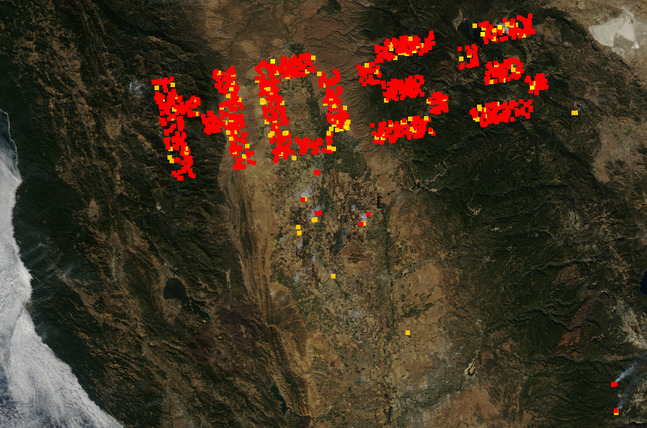
\includegraphics[width=\columnwidth]{diagrams/injection/pixels_800_140.jpg}
    \caption{An injected signal from the attacker manipulates the infrared channels of satellite imagery to create ficticious fires in the resulting dataset.}
    \label{fig:location-injection}
\end{figure}

As global reliance on this data increases, the security implications are becoming increasingly relevant.
Recent news demonstrates that motivated adversaries exist, and are interested in exploiting the decoding and demodulating pipelines.
For example, a recent attack against ViaSat's satellite broadband capabilities exploited side channel vulnerabilities in the terrestrial network, resulting in the receiver stations across Ukraine being permanently disabled; a move coinciding with the Russian invasion of the country~\cite{satcomAnalysis}.

To support a wide range of use cases, raw satellite data is processed into more specialized derived datasets such as for forest fire and storm detection~\cite{nasaFirms,sarikhani2021new}.
This feeds into applications including critical national infrastructure and research-oriented purposes.
The importance of these applications makes attacking the raw data appealing.

Although these applications of satellite data are new, they rely on satellite infrastructure that was launched decades ago.
Since then radio hardware has become more accessible and knowledge of attacks on wireless systems has become more widespread.
Therefore, satellite-derived datasets and the processing systems that create them are now exposed to realistic attacks from far more adversaries -- in particular, data modification attacks from signal injection.
Critical services including NASA's \textit{Fire Information and Resource Management System} (FIRMS) can be affected (shown in Figure~\ref{fig:location-injection}) to trigger false emergency response or mislead crisis analysis.

The security community is becoming increasingly aware that radio overshadowing in a satellite context has the potential to affect critical services.
%\textbf{TODO cite}
As a result, recent countermeasures have been proposed which analyze artifacts of overshadowing on the physical channel to determine the authenticity of the received data~\cite{jedermann2021orbit,oligeri2020past}.
However, the impact of signal overshadowing against currently-deployed satellites, and the real-world consequences on the systems that depend upon their data, have not yet been considered.

\subsection{Contributions}

Specifically, we make the following contributions:

\begin{itemize}
    \item We identify the capability of a modern adversary to affect satellite downlink processing systems using physical-layer attacks;
    \item We illustrate the problem using a full end-to-end case study against NASA's FIRMS service, demonstrating masking of forest fires and generation of fake fires. We further show denial of service and arbitrary code execution attacks on the processing systems themselves;
    \item We discuss the potential impact of similar attacks against other satellite-derived datasets, exploring the effects that an attacker could expect to cause in the real world;
    \item We analyze the feasibility of radio signal injection using commercial off-the-shelf equipment, taking into account the unique constraints of a terrestrial attacker against a highly directional dish;
    \item Finally, we examine the applicability of existing countermeasures, with respect to the unique constraints of this context.
\end{itemize}

At the time of writing, we have been in initial contact with NASA's Direct Readout Laboratory to disclose our findings, and are in the process of compiling a complete vulnerability report.
